% Build:  pdflatex nominal_N1_report.tex   (twice, from this directory)
\documentclass[11pt,a4paper]{article}

\usepackage[margin=2.3cm]{geometry}
\usepackage[T1]{fontenc}
\usepackage{lmodern}
\usepackage{microtype}
\usepackage{amsmath,amssymb}
\usepackage{graphicx}
\usepackage{booktabs}
\usepackage{subcaption}
\usepackage[font=small,labelfont=bf]{caption}
\usepackage{titlesec}
\usepackage[colorlinks=true,linkcolor=black,citecolor=black]{hyperref}

\graphicspath{{../figs/}}

\titleformat{\section}{\normalfont\large\bfseries}{\thesection}{0.7em}{}
\titlespacing*{\section}{0pt}{1.4ex plus .3ex}{0.8ex}

\newcommand{\code}[1]{\texttt{\small #1}}
\newcommand{\Teff}{T_{\mathrm{eff}}}
\newcommand{\vperp}{v_\perp}
\newcommand{\vpar}{v_\parallel}
\setlength{\parskip}{0pt}
\setlength{\textfloatsep}{8pt plus 2pt minus 2pt}
\setlength{\intextsep}{8pt plus 2pt minus 2pt}
\setlength{\floatsep}{8pt plus 2pt minus 2pt}
\setlength{\abovecaptionskip}{4pt}
\setlength{\belowcaptionskip}{0pt}

\title{\vspace{-1.2cm}\textbf{\large Fundamental minority ICRF heating in ITER-EDA}\\[1mm]
\normalsize The nominal $N{=}1$ reference case}
\author{\normalsize F.~Louche}
\date{\normalsize 19 August 2026}

\begin{document}
\maketitle
\vspace{-0.9cm}

\begin{abstract}
\noindent\small
The reference fundamental ITER-EDA case uses the same mass-3 minority at $50\%$
concentration in deuterium as its second-harmonic counterpart, but heated at
$30.45\,$MHz. It settles in $1.0\,$s of physical time at an effective
temperature of $17.25\,$keV against a $12\,$keV bulk, remaining nearly
isotropic at $55.7\%$. Despite absorbing \emph{more} power than the $N{=}2$
case, $2.31$ against $1.82\,$MW/m$^3$, it heats the population as a whole
rather than building a supra-thermal tail, and sheds $92\%$ of that power to
the background ions. It is a mild, ion-drag-dominated equilibrium.
\end{abstract}

\vspace{-0.3cm}
\section{Configuration}

The plasma is identical to the $N{=}2$ reference: a tritium-like minority
(mass 3, $Z{=}1$) in deuterium, both at $50\%$ of
$n_e=1.5\times10^{20}\,$m$^{-3}$, with $T_e=T_i=12\,$keV and $B_0=6\,$T. Only
the wave differs (Table~\ref{tab:setup}) --- fundamental resonance at half the
frequency, a smaller $k_\perp$, and field amplitudes some five times lower. The
velocity domain is correspondingly smaller. Self-collisions use the non-linear
Rosenbluth operator (\code{isc = -1}) with $\theta=0.75$ (\code{icn = 1}).

\begin{table}[h]
\centering\small
\caption{Case parameters. The run terminated on the \code{conv\_diag} criteria
at $t=1.0\,$s after $77\,$s of wall time, twelve times faster than the $N{=}2$
case.}
\label{tab:setup}
\begin{tabular}{@{}llll@{}}
\toprule
harmonic & $N=1$ & grid & $150\times150$, quadratic in $\vperp$ \\
frequency & $30.45\,$MHz & $\vperp^{\max}$ & $2.0\times10^{7}\,$m/s \\
$k_\perp$, $k_\parallel$ & $30$, $2\,$m$^{-1}$ & $\vpar$ range & $[-6,6]\times10^{6}\,$m/s \\
$E_+$ & $(250,100)\,$V/m & minority & mass 3, $Z=1$, $50\%$ \\
$E_-$ & $(750,1)\,$V/m & majority & deuterium, $50\%$ \\
\bottomrule
\end{tabular}
\end{table}

\vspace{-0.2cm}
\section{The steady distribution}

The converged distribution (Fig.~\ref{fig:fout}) is close to a Maxwellian that
has simply been warmed. There is no pronounced perpendicular structure: the
$J_0$-weighted fundamental operator deposits its energy far more broadly in
$\vperp$ than the $J_1$-weighted second harmonic, and the resulting distribution
stays within a few per cent of isotropy throughout.

\begin{figure}[h]
\centering
\begin{subfigure}{0.49\textwidth}\centering
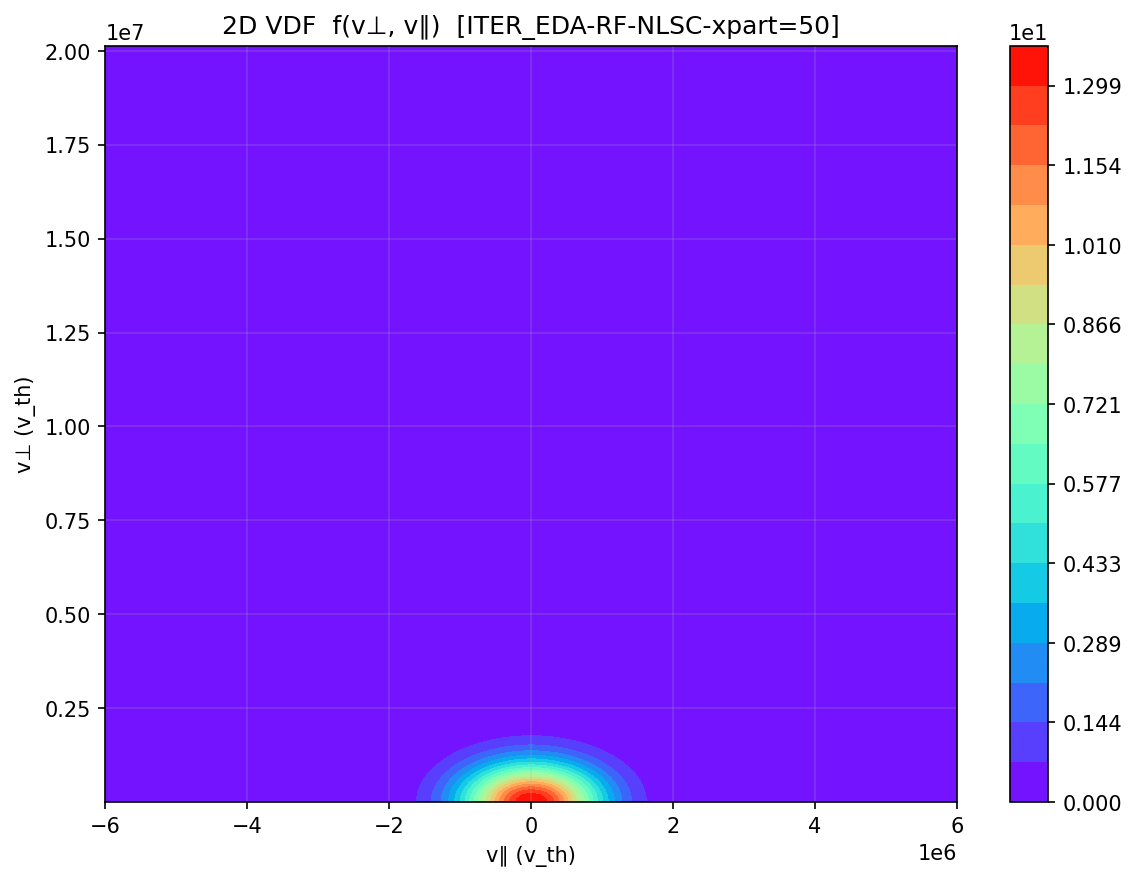
\includegraphics[width=\linewidth]{fout-ITER_EDA-RF-NLSC-xpart=50.png}
\caption{$f(\vperp,\vpar)$}
\end{subfigure}\hfill
\begin{subfigure}{0.49\textwidth}\centering
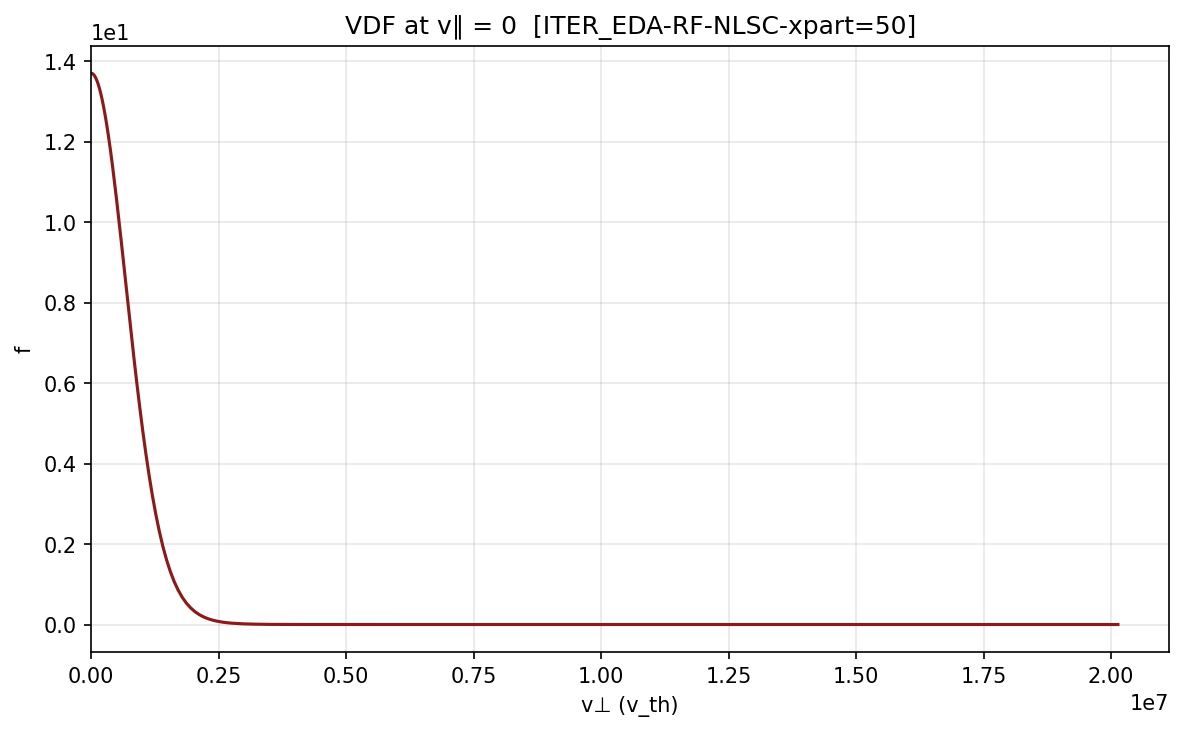
\includegraphics[width=\linewidth]{fout_at_vpar0-ITER_EDA-RF-NLSC-xpart=50.png}
\caption{cut at $\vpar=0$}
\end{subfigure}
\caption{Converged minority distribution. Compare with the second-harmonic
case, whose contours are strongly elongated in $\vperp$; here they are almost
circular.}
\label{fig:fout}
\end{figure}

\vspace{-0.2cm}
\section{Bulk heating rather than tail formation}

The clearest signature of the difference between the two harmonics is not
$\Teff$ but its relation to the density-characteristic temperature $T_n$. Here
$\Teff$ rises from $12.53$ to $17.25\,$keV and $T_n$ follows it closely, from
$12.46$ to $16.23\,$keV (Fig.~\ref{fig:evol}): the two agree to $6\%$, meaning
the entire population has been heated. In the $N{=}2$ case the same pair reads
$32.59$ and $13.73\,$keV --- a factor $2.4$ apart --- because there the energy
sits in a tail that the second moment sees and the bulk does not.

The anisotropy tells the same story from another angle, rising only from
$51.5\%$ to $55.7\%$ against the second harmonic's $73.9\%$. Both quantities
saturate by $t\simeq0.6\,$s.

\begin{figure}[h]
\centering
\begin{subfigure}{0.49\textwidth}\centering
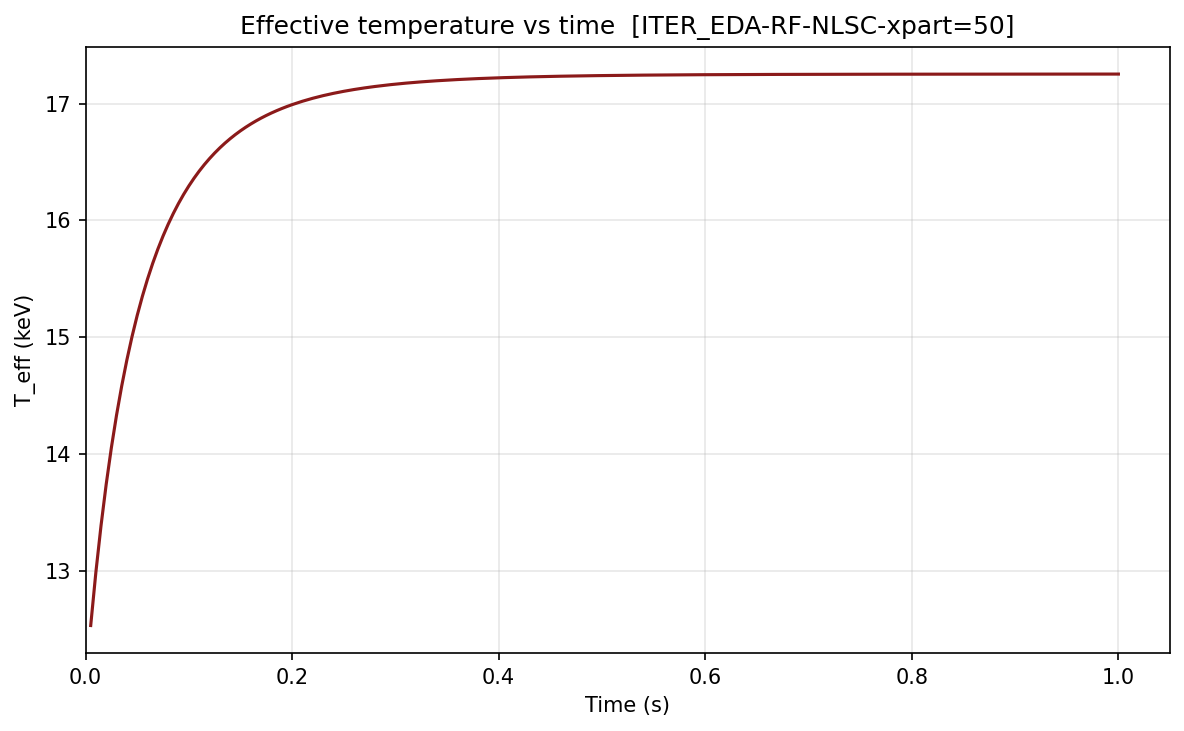
\includegraphics[width=\linewidth]{Teff_vs_time-ITER_EDA-RF-NLSC-xpart=50.png}
\caption{effective temperature}
\end{subfigure}\hfill
\begin{subfigure}{0.49\textwidth}\centering
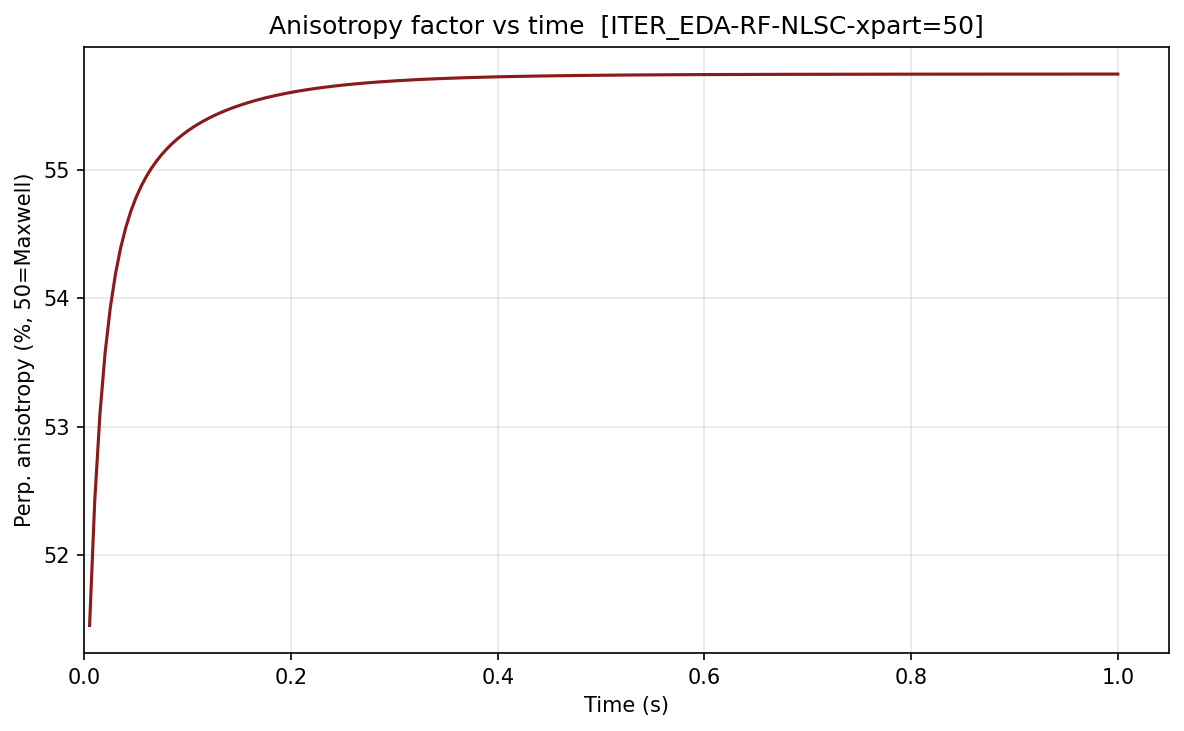
\includegraphics[width=\linewidth]{anisotropy_vs_time-ITER_EDA-RF-NLSC-xpart=50.png}
\caption{perpendicular anisotropy}
\end{subfigure}
\caption{Approach to steady state; $50\%$ anisotropy would be isotropic.}
\label{fig:evol}
\end{figure}

\vspace{-0.2cm}
\section{Power balance and timescales}

The RF supplies $2.3118\,$MW/m$^3$ and the collisions remove the same to within
$0.001\%$ (Fig.~\ref{fig:power}). The split is overwhelmingly to the ions:
$2.118\,$MW/m$^3$ against $0.194$ to the electrons, or $92{:}8$. With a critical
energy of $E_c\simeq106\,$keV and a tail at $17\,$keV, the minority sits deep in
the ion-drag regime and never approaches the ion-to-electron transition that the
second harmonic reaches at $59{:}41$.

Self-collisions again carry no net energy, moving $0.304\,$MW/m$^3$ from the
perpendicular direction to the parallel and closing to $0.004\%$. It is worth
noting that this is \emph{larger} than the $0.176\,$MW/m$^3$ of the $N{=}2$
case, even though neglecting self-collisions costs only $5.6\%$ here against
$144\%$ there: the magnitude of the self-collision term is no guide to how much
the answer depends on it.

\begin{figure}[h]
\centering
\begin{subfigure}{0.49\textwidth}\centering
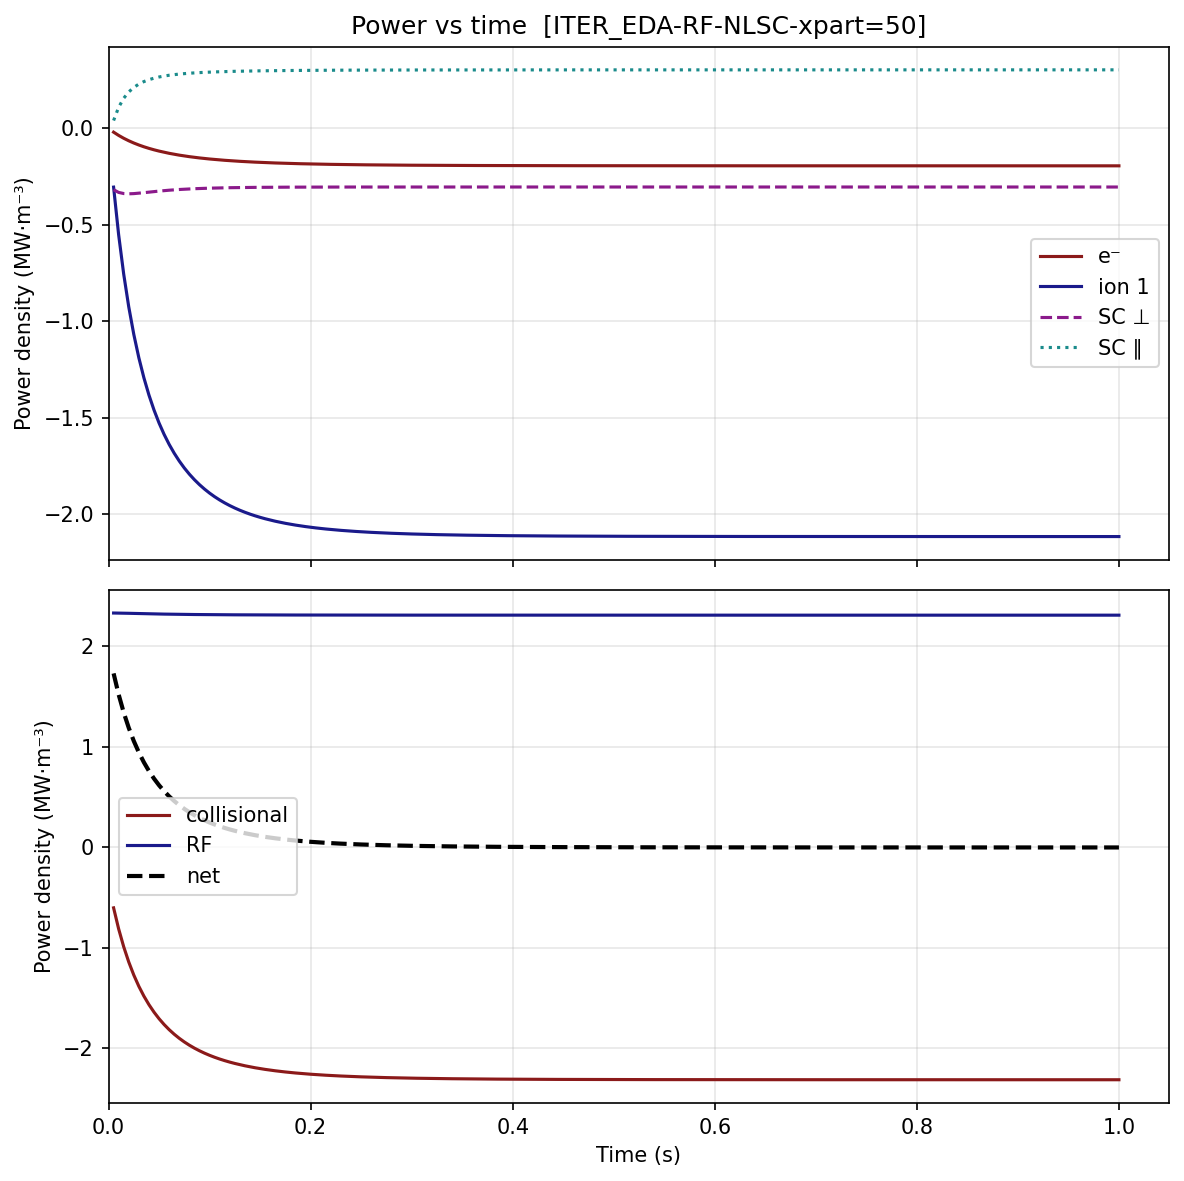
\includegraphics[width=\linewidth]{power_vs_time-ITER_EDA-RF-NLSC-xpart=50.png}
\caption{power balance}
\end{subfigure}\hfill
\begin{subfigure}{0.49\textwidth}\centering
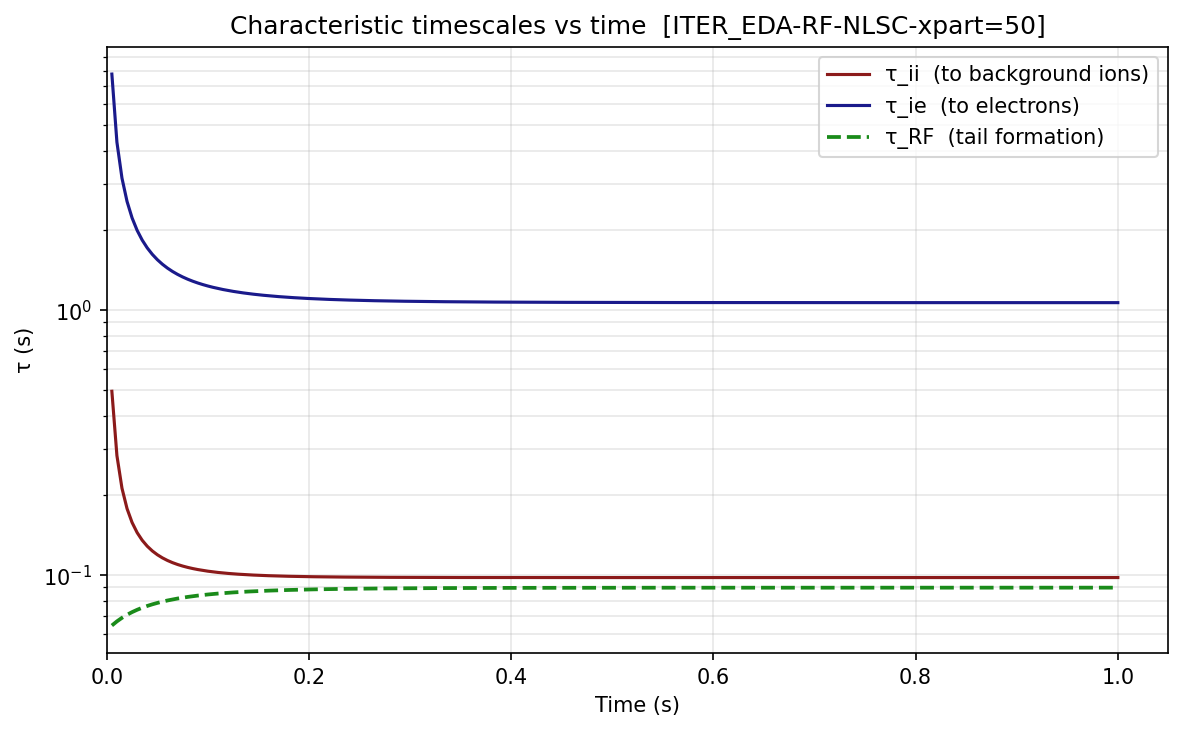
\includegraphics[width=\linewidth]{timescales_vs_time-ITER_EDA-RF-NLSC-xpart=50.png}
\caption{characteristic timescales}
\end{subfigure}
\caption{Power channels and the effective timescales $\tau = n\Teff/P$. The
identity $1/\tau_{\rm RF}=1/\tau_{ii}+1/\tau_{ie}$ holds to $0.001\%$.}
\label{fig:power}
\end{figure}

As timescales, the RF fills on $\tau_{\rm RF}=0.090\,$s and the ions drain on
$\tau_{ii}=0.098\,$s --- the two are within $8\%$, so the equilibrium is
essentially a balance between the RF and ion drag alone. Electron drag, at
$\tau_{ie}=1.07\,$s, is an order of magnitude slower and barely participates.
That near-equality of $\tau_{\rm RF}$ and $\tau_{ii}$, against the factor $1.7$
separating them at $N{=}2$, is why the fundamental sustains so much less
supra-thermal population.

\vspace{-0.2cm}
\section{Summary and numerical quality}

\begin{table}[h]
\centering\small
\caption{Steady-state results, with the $N{=}2$ reference alongside.}
\begin{tabular}{@{}lrr@{}}
\toprule
 & $N{=}1$ & $N{=}2$ \\
\midrule
$\Teff$                  & $17.25\,$keV   & $32.59\,$keV \\
$T_n$                    & $16.23\,$keV   & $13.73\,$keV \\
anisotropy               & $55.75\%$      & $73.86\%$ \\
$P_{\rm RF}$             & $2.3118\,$MW/m$^3$ & $1.8166\,$MW/m$^3$ \\
ion\,:\,electron split   & $92:8$         & $59:41$ \\
$\tau_{\rm RF}$          & $0.0897\,$s    & $0.2156\,$s \\
$\tau_{ii}$, $\tau_{ie}$ & $0.098$, $1.068\,$s & $0.364$, $0.528\,$s \\
convergence              & $1.0\,$s       & $12.5\,$s \\
\bottomrule
\end{tabular}
\end{table}

Numerically this is the better-behaved of the two cases. It stops on the
convergence criteria after $1.0\,$s, with a residual drift in $\Teff$ of
$0.008\%$ over the final quarter of the run and a density change of $+0.003\%$
--- forty times smaller than the $N{=}2$ case, since the self-collision
operator's slow particle gain has far less time to accumulate. Wall truncation
of $f$ is $9.6\times10^{-27}$ of the peak in $\vperp$ and $6.2\times10^{-13}$ in
$\vpar$, so the smaller velocity domain used here is amply sufficient.

\vspace{0.2cm}
\noindent\footnotesize
Case \code{nominal\#1}; figures from \code{figs/}, generated by
\code{fp2d\_plot.py} from the traces in \code{results/}.

\end{document}
